\chapter{التركيب الضوئي والتغذي الذاتي}\label{ch:b1:photosynthesis}

كل غرام من الكربون في الأرنب والبلوطة والقارئ وهذه الصفحة كان يومًا
ثاني أكسيد كربون في الهواء، وقد ثبّتته \omterm{def:b1:flowering-plant-organization:organs}{ورقة} --- أو طحلب، أو بكتيريا
زرقاء --- سكرًا، بطاقة ضوء الشمس. والتفاعل، ستة $\mathrm{CO_2}$ وستة
ماء إلى غلوكوز واحد وستة أكسجين، صعودي بمقدار \qty{2870}{kJ/mol}؛
\omterm{def:b1:flowering-plant-organization:organs}{والورقة} تجريه بشطر الماء بالضوء، وخزن الإلكترونات على NADPH والطاقة
على \omterm{def:b1:water-small-molecules:atp}{ATP}، ثم إنفاق الاثنين في دورة تبني السكر. يصف هذا الفصل
\omterm{def:b1:photosynthesis:chloroplast}{البلاستيدة الخضراء}، والأصبغة \omterm{prop:b1:photosynthesis:lightreactions}{والتفاعلات الضوئية} التي تصنع \omterm{def:b1:water-small-molecules:atp}{ATP} وNADPH،
\omterm{def:b1:photosynthesis:fixation}{ودورة كالفن} التي تثبّت الكربون، والتسرب المسمى \omterm{prop:b1:photosynthesis:photorespiration}{التنفس الضوئي}
والتصميمين اللذين يسدانه، وما \omterm{def:b1:photosynthesis:autotrophy}{التغذي الذاتي} عمومًا.

\section{البلاستيدة الخضراء وأصبغتها}

\begin{definition}[البلاستيدة الخضراء]\label{def:b1:photosynthesis:chloroplast}
\emph{البلاستيدة الخضراء}\index{بلاستيدة خضراء} عضية عدسية الشكل
طولها \qtyrange{3}{10}{\micro m} يحدها غشاءا غلاف؛ وداخلها،
\emph{السدى}\index{سدى}، يحمل \omterm{def:b1:enzymes:enzyme}{إنزيمات} تثبيت الكربون، وحبيبات \omterm{def:b1:carbohydrates:polysaccharide}{نشا}،
وريبوزومات، \omterm{def:b1:nucleic-acids:chain}{وDNA} حلقيًا؛ وضمن السدى جملة \omterm{def:b1:membranes-transport:membrane}{أغشية} ثالثة، هي
\emph{الثايلاكويدات}\index{ثايلاكويد}، تكوّن أكياسًا مفلطحة مكدسة في
\emph{أكداس} توصلها صفائح، وتحيط \emph{بلمعة ثايلاكويدية} واحدة
متصلة. \omterm{prop:b1:photosynthesis:lightreactions}{والتفاعلات الضوئية} تجري في الغشاء الثايلاكويدي؛ وتثبيت
الكربون في السدى. \omterm{def:b1:cell-unit-of-life:cell}{وخلية} \omterm{def:b1:flowering-plant-organization:organs}{الورقة} تحمل \qtyrange{20}{100}{} \omterm{def:b1:eukaryotic-cell:plastid}{بلاستيدة}
خضراء؛ والمليمتر المربع من الورق نصف مليون.
\end{definition}

\begin{omfigure}
\begin{tikzpicture}
  \node[anchor=south west, inner sep=0] (img) at (0,0)
    {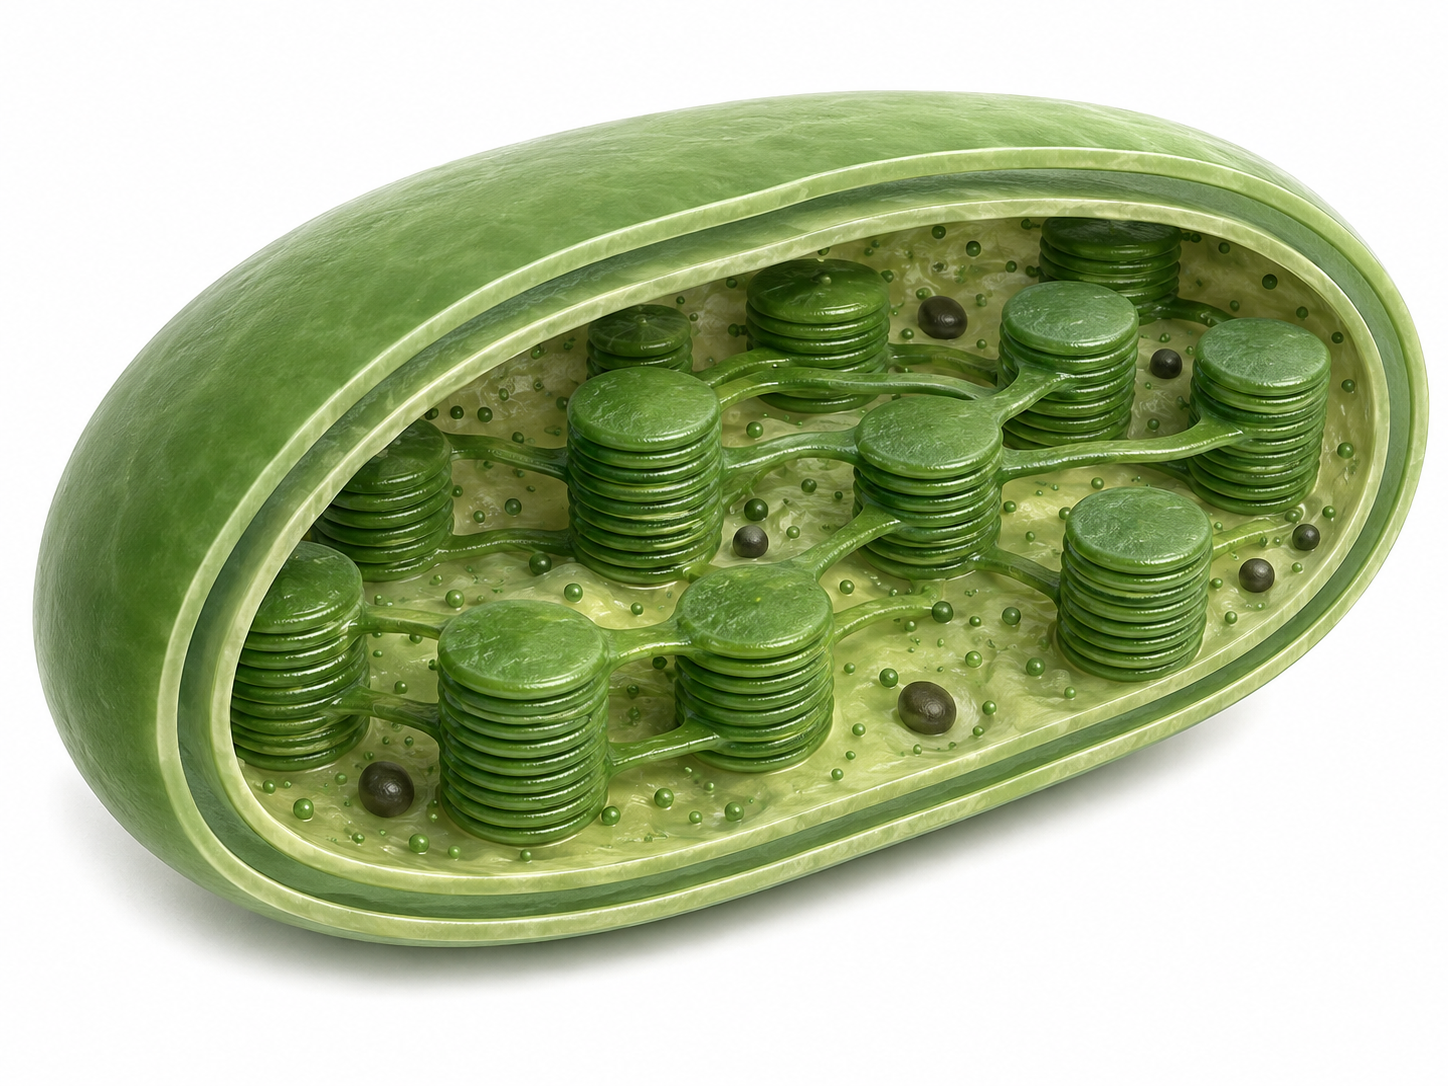
\includegraphics[width=0.56\linewidth]{images/book3/ai/fig-chloroplast-cutaway.png}};
  \begin{scope}[x={(img.south east)}, y={(img.north west)},
      every node/.style={font=\small}]
    \draw[omDef, thick] (0.12,0.50) -- (-0.03,0.66) node[left, align=right] {غشاءا الغلاف\\ الاثنان};
    \draw[omDef, thick] (0.48,0.60) -- (0.48,1.08) node[above] {كدس: رزمة من الثايلاكويدات};
    \draw[omDef, thick] (0.62,0.52) -- (1.03,0.62) node[right] {صفيحة سدوية};
    \draw[omDef, thick] (0.35,0.24) -- (-0.03,0.16) node[left] {سدى};
    \draw[omDef, thick] (0.86,0.50) -- (1.03,0.40) node[right] {حبيبة نشا};
  \end{scope}
\end{tikzpicture}

{\small \omterm{def:b1:photosynthesis:chloroplast}{بلاستيدة خضراء} مشقوقة. غشاءا غلاف حول \omterm{def:b1:photosynthesis:chloroplast}{السدى}؛ وفي الداخل
أكداس من \omterm{def:b1:photosynthesis:chloroplast}{الثايلاكويدات} توصلها صفائح وتحيط بلمعة واحدة. والضوء يُلتقط
في الغشاء الثايلاكويدي والسكر يُصنع في \omterm{def:b1:photosynthesis:chloroplast}{السدى}.}
\end{omfigure}

\begin{definition}[أصبغة التركيب الضوئي]\label{def:b1:photosynthesis:pigments}
\emph{اليخضور}\index{يخضور} $a$ و$b$ حلقتان بورفيرينيتان حول ذرة
مغنيزيوم بذيل كاره للماء طويل يرسّيهما في الغشاء الثايلاكويدي؛ وهما
يمتصان الضوء الأزرق (\qtyrange{430}{450}{nm}) والأحمر
(\qtyrange{640}{680}{nm}) ويعكسان الأخضر.
و\emph{الكاروتينويدات}\index{كاروتينويد} (وهي إيزوبرينويدات،
\cref{ch:b1:lipids}) تمتص الضوء الأزرق المخضر وتمرر الطاقة إلى
اليخضور، وتحميه بإخماد الإثارة الزائدة. وبضع مئات من جزيئات الأصبغة،
محمولة على \omterm{def:b1:proteins:peptide}{بروتينات} بوصفها \emph{هوائيًا} (معقد حصاد الضوء)، تقمع
طاقة كل فوتون ممتص إلى زوج خاص واحد من جزيئات اليخضور $a$، هو
\emph{مركز التفاعل}، حيث تتحول إلى كيمياء.
\end{definition}

\begin{omfigure}
\begin{tikzpicture}
\begin{axis}[
  width=0.88\linewidth, height=6.2cm,
  axis x line=bottom, axis y line=left,
  xmin=400, xmax=720, ymin=0, ymax=1.1,
  xlabel={طول الموجة (\unit{nm})}, ylabel={الامتصاص، أو المعدل (نسبي)},
  xlabel style={font=\small, at={(axis description cs:0.5,-0.12)}, anchor=north},
  ylabel style={font=\small},
  tick label style={font=\small}, xtick={400,450,500,550,600,650,700}, ytick={0,0.5,1},
  legend style={font=\small, at={(0.5,0.98)}, anchor=north, draw=none},
  clip=false,
]
\addplot[very thick, omDef, domain=400:720, samples=160] {exp(-((x-430)/18)^2) + 0.85*exp(-((x-662)/14)^2) + 0.05};
\addlegendentry{امتصاص اليخضور $a$}
\addplot[very thick, omExo, domain=400:720, samples=160] {0.7*exp(-((x-455)/20)^2) + 0.5*exp(-((x-645)/14)^2) + 0.05};
\addlegendentry{امتصاص اليخضور $b$}
\addplot[very thick, omProp, domain=400:720, samples=160] {0.75*exp(-((x-470)/25)^2) + 0.05};
\addlegendentry{امتصاص الكاروتينويدات}
\addplot[very thick, dashed, omThm, domain=400:720, samples=160] {0.9*exp(-((x-440)/30)^2) + 0.35*exp(-((x-520)/50)^2) + 0.85*exp(-((x-660)/22)^2) + 0.1};
\addlegendentry{طيف الفعل: معدل إطلاق $\mathrm{O_2}$}
\end{axis}
\end{tikzpicture}

{\small أطياف امتصاص أصناف الأصبغة الثلاثة وطيف فعل التركيب الضوئي
(أي معدل إطلاق الأكسجين عند كل طول موجة). وطيف الفعل يتبع اليخضورين،
ويملأ \omterm{def:b1:photosynthesis:pigments}{الكاروتينويدات} فراغه في الأزرق المخضر: فكل صباغ يمتص يسهم.}
\end{omfigure}

\begin{proposition}[طيف الفعل يتبع الأصبغة]\label{prop:b1:photosynthesis:engelmann}
يقود التركيبَ الضوئي الضوءُ الذي تمتصه الأصبغة: فهو أسرع ما يكون في
الضوء الأحمر والأزرق، وأضعفه في الأخضر.
\end{proposition}
\begin{proof}[شواهد]
وضع إنغلمان (1882) خيطًا من طحلب عبر طيف مسقط تحت مجهره وأضاف
بكتيريا تسعى إلى الأكسجين: فتجمعت حيث يسقط الضوء الأحمر والأزرق، لا
في الأخضر (المستعاد من كتاب المرحلة الثانوية). ومقيسًا بمسرى أكسجين،
يعطي المعدل عند كل طول موجة طيف الفعل السابق، وهو يتبع امتصاص
اليخضورين؛ والفائض في الأزرق المخضر إسهام \omterm{def:b1:photosynthesis:pigments}{الكاروتينويدات}، وهو يبين
أنها تمرر طاقتها.
\end{proof}

\section{التفاعلات الضوئية}

\begin{proposition}[ماذا تفعل التفاعلات الضوئية]\label{prop:b1:photosynthesis:lightreactions}
\index{التفاعلات الضوئية}
في الغشاء الثايلاكويدي تُستعمل طاقة الضوء لنقل الإلكترونات من الماء
إلى $\mathrm{NADP^+}$ --- صعودًا، ضد فرق كمون أكسدة وإرجاع قدره
\qty{1.1}{V} --- ولضخ البروتونات إلى اللمعة:
\[
2\,\mathrm{H_2O} + 2\,\mathrm{NADP^+} + 3\,\mathrm{ADP} + 3\,\mathrm{P_i}
\xrightarrow{\ 8\ \text{فوتونات}\ }
\mathrm{O_2} + 2\,\mathrm{NADPH} + 2\,\mathrm{H^+} + 3\,\mathrm{ATP} .
\]
والأكسجين المطلق أكسجين الماء لا أكسجين ثاني أكسيد الكربون؛ وNADPH
يحمل القدرة المرجعة \omterm{def:b1:water-small-molecules:atp}{وATP} يحمل الطاقة التي ستنفقها \omterm{def:b1:photosynthesis:fixation}{دورة كالفن}.
\end{proposition}
\begin{proof}[شواهد]
بيّن هِل (1937) أن بلاستيدات خضراء معزولة في الضوء تطلق أكسجينًا في
غياب $\mathrm{CO_2}$ إذا وُجد متقبل إلكترونات اصطناعي: فشطر الماء
منفصل عن تثبيت الكربون. وأطعم روبن وكامن (1941) طحالب ماءً موسومًا
بأكسجين ثقيل فوجدا الوسم في $\mathrm{O_2}$ المطلق، ولم يجداه حين كان
الوسم في $\mathrm{CO_2}$. ووجد إمرسون (1957) أن الضوء الأحمر عند
\qty{700}{nm}، وهو شبه عديم النفع وحده، مع الضوء عند \qty{680}{nm}
يعطيان معًا أكثر من مجموع معدليهما المنفصلين: فلا بد من نظامين ضوئيين
مختلفي الأصبغة يعملان على التسلسل.
\end{proof}

\begin{definition}[النظامان الضوئيان ومخطط Z]\label{def:b1:photosynthesis:zscheme}
\index{نظام ضوئي}\index{مخطط Z}
يقع \emph{نظامان ضوئيان} في الغشاء الثايلاكويدي. ففي \emph{النظام
الضوئي الثاني} (PSII، ومركز تفاعله P680) يرفع فوتون ممتص إلكترونًا من
الزوج الخاص إلى طاقة عالية؛ فيغادر الإلكترون، ويأخذ P680 المؤكسد،
وهو أقوى المؤكسدات الحيوية، إلكترونًا من الماء: إذ يشطر عنقود منغنيز
جزيئي ماء إلى $\mathrm{O_2}$، وأربعة بروتونات (تُطلق في اللمعة)،
وأربعة إلكترونات، فوتونًا فوتونًا. ثم يهبط الإلكترون \emph{سلسلة نقل
إلكترونات} --- البلاستوكينون، و\emph{معقد السيتوكروم $b_6f$}،
والبلاستوسيانين --- والطاقة التي يفقدها تضخ بروتونات إلى اللمعة. وفي
\emph{النظام الضوئي الأول} (PSI، وP700) يرفعه فوتون ثانٍ من جديد،
إلى كمون منخفض بما يكفي لإرجاع الفيريدوكسين ثم إرجاع
$\mathrm{NADP^+}$ إلى NADPH. ومرسومًا على سلم كمون الأكسدة والإرجاع
يكون المسار حرف Z: صعودان بالضوء، وهبوطان بالكيمياء.
\end{definition}

\begin{omfigure}
\begin{tikzpicture}[font=\footnotesize, >=Stealth, line cap=round,
  st/.style={draw, thick, rounded corners=2pt, inner sep=2pt}]
  % redox potential axis (vertical, more negative up)
  \draw[->, thick] (0,0) -- (0,6.4) node[above, font=\small] {كمون الأكسدة والإرجاع $E'_0$ (V)};
  \foreach \y/\l in {0.4/{$+1.0$}, 1.9/{$+0.5$}, 3.4/{$0$}, 4.9/{$-0.5$}, 6.0/{$-0.9$}} { \draw (-0.1,\y) -- (0.1,\y) node[left, xshift=-4pt] {\l}; }
  % PSII
  \node[st, fill=omDef!15] (h2o) at (1.7,1.0) {$\mathrm{H_2O}$};
  \node[st, fill=omDef!25] (p680) at (2.9,0.35) {P680};
  \node[st, fill=omDef!25] (p680s) at (2.9,5.7) {P680*};
  \draw[->, thick] (h2o) -- (p680);
  \node[anchor=west, font=\scriptsize] at (3.5,0.35) {$\to \mathrm{O_2} + 4\,\mathrm{H^+}$ إلى اللمعة};
  \draw[->, very thick, omProp] (p680) -- (p680s) node[pos=0.45, right, align=left] {فوتون\\ (\qty{680}{nm})};
  % chain
  \node[st, fill=omThm!15] (pq) at (4.2,4.4) {PQ};
  \node[st, fill=omThm!15] (b6f) at (5.4,3.6) {سيتوكروم $b_6f$};
  \node[st, fill=omThm!15] (pc) at (6.5,2.8) {PC};
  \draw[->, thick] (p680s) -- (pq); \draw[->, thick] (pq) -- (b6f); \draw[->, thick] (b6f) -- (pc);
  \node[anchor=south west, align=left, font=\scriptsize, omThm] at (4.75,4.15) {$\mathrm{H^+}$ مضخوخة\\ إلى اللمعة};
  % PSI
  \node[st, fill=omExo!25] (p700) at (7.7,2.3) {P700};
  \node[st, fill=omExo!25] (p700s) at (7.7,6.0) {P700*};
  \draw[->, thick] (pc) -- (p700);
  \draw[->, very thick, omProp] (p700) -- (p700s) node[pos=0.45, right, align=left] {فوتون\\ (\qty{700}{nm})};
  \node[st, fill=omThm!15] (fd) at (9.1,5.2) {Fd};
  \node[st, fill=omExo!15] (nadp) at (10.5,4.6) {NADPH};
  \draw[->, thick] (p700s) -- (fd); \draw[->, thick] (fd) -- (nadp);
  \node[anchor=north, font=\scriptsize] at (10.5,4.3) {$E'_0 = \qty{-0.32}{V}$};
  % cyclic flow
  \draw[->, thick, dashed, gray] (fd) .. controls (7.2,5.5) and (4.4,5.5) .. (pq.north);
  \node[gray, font=\scriptsize, anchor=south] at (5.6,5.45) {جريان حلقي (ATP فقط)};
\end{tikzpicture}

{\small \omterm{def:b1:photosynthesis:zscheme}{مخطط Z}. الإلكترونات المأخوذة من الماء عبر P680 يرفعها فوتون،
فتهبط سلسلة تضخ البروتونات، ثم يرفعها P700 من جديد فتنتهي على NADPH.
والمحور الشاقولي كمون أكسدة وإرجاع، يزداد سلبية صعودًا: فالضوء يتولى
الصعود والكيمياء الهبوط.}
\end{omfigure}

\begin{theorem}[تركيب ATP تناضحيًا كيميائيًا]\label{thm:b1:photosynthesis:chemiosmosis}
\index{التناضح الكيميائي}\index{سنتاز ATP}
البروتونات المحررة بشطر الماء والمضخوخة بمعقد السيتوكروم $b_6f$
تتراكم في لمعة \omterm{def:b1:photosynthesis:chloroplast}{الثايلاكويد}، التي تهبط في الضوء إلى pH 5 بينما يرتفع
\omterm{def:b1:photosynthesis:chloroplast}{السدى} إلى pH 8: أي فرق ثلاث وحدات، وقوة محركة للبروتون تناهز
\qty{0.18}{V}، تكافئ \qty{17}{kJ} لكل مول بروتون. و\emph{\omterm{thm:b1:photosynthesis:chemiosmosis}{سنتاز ATP}}،
وهو محرك دوّار يعبر الغشاء الثايلاكويدي، يدع البروتونات تجري راجعة
إلى \omterm{def:b1:photosynthesis:chloroplast}{السدى} ويستعمل الطاقة لفسفرة ADP: بنحو \qty{4}{H^+} لكل \omterm{def:b1:water-small-molecules:atp}{ATP}.
ونقل الإلكترونات وتركيب \omterm{def:b1:water-small-molecules:atp}{ATP} لا يقترنان إلا عبر هذا التدرج (نظرية
ميتشل التناضحية الكيميائية، 1961).
\end{theorem}
\begin{proof}[شواهد]
نقع ياغندورف (1966) ثايلاكويدات في الظلام في حمام حمضي (pH 4) حتى
صارت لمعتها حمضية، ثم نقلها فجأة إلى pH 8 مع ADP وفوسفات: فصُنع \omterm{def:b1:water-small-molecules:atp}{ATP}
في الظلام، من التدرج وحده. وفواصل الاقتران --- وهي حموض ضعيفة منحلة
في \omterm{def:b1:lipids:fattyacid}{الدهن} تحمل البروتونات عبر \omterm{def:b1:membranes-transport:membrane}{الأغشية} --- تلغي تركيب \omterm{def:b1:water-small-molecules:atp}{ATP} بينما يستمر
نقل الإلكترونات وإطلاق الأكسجين، بل ويتسارعان. \omterm{thm:b1:photosynthesis:chemiosmosis}{وسنتاز ATP} المعزول
المعاد تركيبه في حويصلات اصطناعية يصنع \omterm{def:b1:water-small-molecules:atp}{ATP} حين يُفرض تدرج pH، ويحلمه
\omterm{def:b1:water-small-molecules:atp}{ATP} ليضخ البروتونات حين لا يُفرض. وقد شوهد دوران \omterm{def:b1:enzymes:enzyme}{الإنزيم} منذ ذلك
الحين مباشرة، جزيئًا جزيئًا، تحت المجهر.
\end{proof}

\begin{example}[الجريان الحلقي وغير الحلقي]\label{ex:b1:photosynthesis:cyclic}
المسار الخطي من الماء إلى NADPH يعطي، لكل $\mathrm{O_2}$، جزيئي
NADPH ونحو ثلاثة \omterm{def:b1:water-small-molecules:atp}{ATP}؛ \omterm{def:b1:photosynthesis:fixation}{ودورة كالفن} تحتاج إلى نسبة ثلاثة \omterm{def:b1:water-small-molecules:atp}{ATP} إلى
جزيئي NADPH بالضبط، وسائر أعمال \omterm{def:b1:eukaryotic-cell:plastid}{البلاستيدة} تحتاج إلى \omterm{def:b1:water-small-molecules:atp}{ATP} أكثر. وحين
يقصر \omterm{def:b1:water-small-molecules:atp}{ATP} تعود الإلكترونات من الفيريدوكسين إلى البلاستوكينون بدل أن
تذهب إلى $\mathrm{NADP^+}$ (وهي \emph{الفسفرة الضوئية الحلقية}):
فيعمل PSI وحده، يضخ البروتونات ويصنع \omterm{def:b1:water-small-molecules:atp}{ATP} بلا أكسجين ولا NADPH.
والنمطان موزونان بحسب الطلب.
\end{example}

\section{دورة كالفن}

\begin{definition}[تثبيت الكربون]\label{def:b1:photosynthesis:fixation}
\index{دورة كالفن}\index{روبيسكو}
تثبّت \emph{دورة كالفن} في \omterm{def:b1:photosynthesis:chloroplast}{السدى} $\mathrm{CO_2}$ سكرًا على ثلاث
مراحل. \emph{التثبيت}: يضيف \emph{روبيسكو} (كربوكسيلاز/أوكسيجيناز
الربولوز ثنائي الفوسفات) $\mathrm{CO_2}$ إلى الربولوز 1،5-ثنائي
الفوسفات (RuBP، خمس ذرات كربون)، فينشطر الناتج السداسي في الحال إلى
جزيئي 3-فوسفوغليسيرات (3-PGA، ثلاث ذرات كربون).
\emph{والإرجاع}: يُفسفَر كل 3-PGA بجزيء \omterm{def:b1:water-small-molecules:atp}{ATP} ويُرجَع بجزيء NADPH إلى
غليسرألدهيد-3-فوسفات (G3P)، وهو أول سكر. \emph{والتجديد}: يُعاد ترتيب
خمسة من كل ستة G3P، بكلفة \omterm{def:b1:water-small-molecules:atp}{ATP}، إلى ثلاثة RuBP، ويغادر واحد الدورة
ناتجًا صافيًا. والنسب المولية من أجل G3P واحد (ثلاث ذرات كربون) هي
\[
3\,\mathrm{CO_2} + 9\,\mathrm{ATP} + 6\,\mathrm{NADPH} + 6\,\mathrm{H^+}
\to \text{G3P} + 9\,\mathrm{ADP} + 8\,\mathrm{P_i} + 6\,\mathrm{NADP^+} ;
\]
وجزيئا G3P يصنعان غلوكوزًا واحدًا: أي \qty{18}{} \omterm{def:b1:water-small-molecules:atp}{ATP} و\qty{12}{NADPH} لكل غلوكوز.
\end{definition}

\begin{omfigure}
\begin{tikzpicture}[font=\footnotesize, >=Stealth, line cap=round,
  box/.style={draw, thick, rounded corners=3pt, minimum height=8mm, align=center, fill=white}]
  \node[box, fill=omDef!15] (rubp) at (0,2.6) {3 RuBP\\ ($3\times$ C5)};
  \node[box, fill=omDef!15] (pga) at (5.0,2.6) {6 3-PGA\\ ($6\times$ C3)};
  \node[box, fill=omDef!15] (g3p) at (5.0,-0.4) {6 G3P\\ ($6\times$ C3)};
  \node[box, fill=omExo!20] (out) at (9.2,-0.4) {يخرج 1 G3P\\ (الكسب الصافي: 3 كربون)};
  \draw[->, very thick, omThm] (rubp) -- (pga) node[midway, above, align=center] {التثبيت (روبيسكو)\\ $+\,3\,\mathrm{CO_2}$};
  \draw[->, very thick, omThm] (pga) -- (g3p) node[midway, right, align=left] {الإرجاع\\ $6\,\mathrm{ATP}$، $6\,\mathrm{NADPH}$};
  \draw[->, very thick, omThm] (g3p) -- (out);
  \draw[->, very thick, omThm] (g3p) -| (rubp);
  \node[anchor=north, align=center, omThm] at (2.4,-0.95) {التجديد: 5 G3P $\to$ 3 RuBP\\ $3\,\mathrm{ATP}$};
  \node[anchor=north, align=center, gray] at (4.6,-1.7) {لكل دورة (ثلاثة $\mathrm{CO_2}$): 9 ATP، و6 NADPH، وكسب G3P واحد\\ ولدورتين: غلوكوز واحد، و18 ATP، و12 NADPH};
\end{tikzpicture}

{\small \omterm{def:b1:photosynthesis:fixation}{دورة كالفن} من أجل ثلاثة جزيئات $\mathrm{CO_2}$: ثلاثة RuBP
تُثبَّت في ستة 3-PGA، تُرجَع إلى ستة G3P، يغادر منها واحد وتجدد
خمسة منها جزيئات RuBP الثلاثة. والكربون محفوظ في كل خطوة
($15 + 3 = 18 = 3 + 15$).}
\end{omfigure}

\begin{proposition}[شواهد كالفن]\label{prop:b1:photosynthesis:calvin}
أول ناتج مستقر لتثبيت $\mathrm{CO_2}$ هو 3-فوسفوغليسيرات، والمتقبل
هو الربولوز ثنائي الفوسفات.
\end{proposition}
\begin{proof}[شواهد]
أضاء كالفن وبنسون (1948--1954) طحالب في دورق مسطح («المصاصة»)،
وحقنا $\mathrm{^{14}CO_2}$، وقتلا عينات في كحول يغلي بعد ثوان؛ وبيّن
الاستشراب الورقي الثنائي البعد والتصوير الإشعاعي الذاتي أين كان
الوسم. فبعد خمس ثوان كان جله في 3-PGA؛ والتعريضات الأطول نشرته عبر
فوسفات السكريات ثم إلى السكروز \omterm{def:b1:carbohydrates:polysaccharide}{والنشا}. وحين أُزيل $\mathrm{CO_2}$
فجأة تراكم RuBP وهبط 3-PGA؛ وحين أُطفئ الضوء تراكم 3-PGA وهبط RuBP
--- فجزيء RuBP هو المتقبل الذي يستهلكه \omterm{def:b1:photosynthesis:fixation}{التثبيت}، و3-PGA هو الناتج الذي
يستهلكه \omterm{def:b1:water-small-molecules:atp}{ATP} وNADPH الآتيان من الضوء.
\end{proof}

\begin{omfigure}
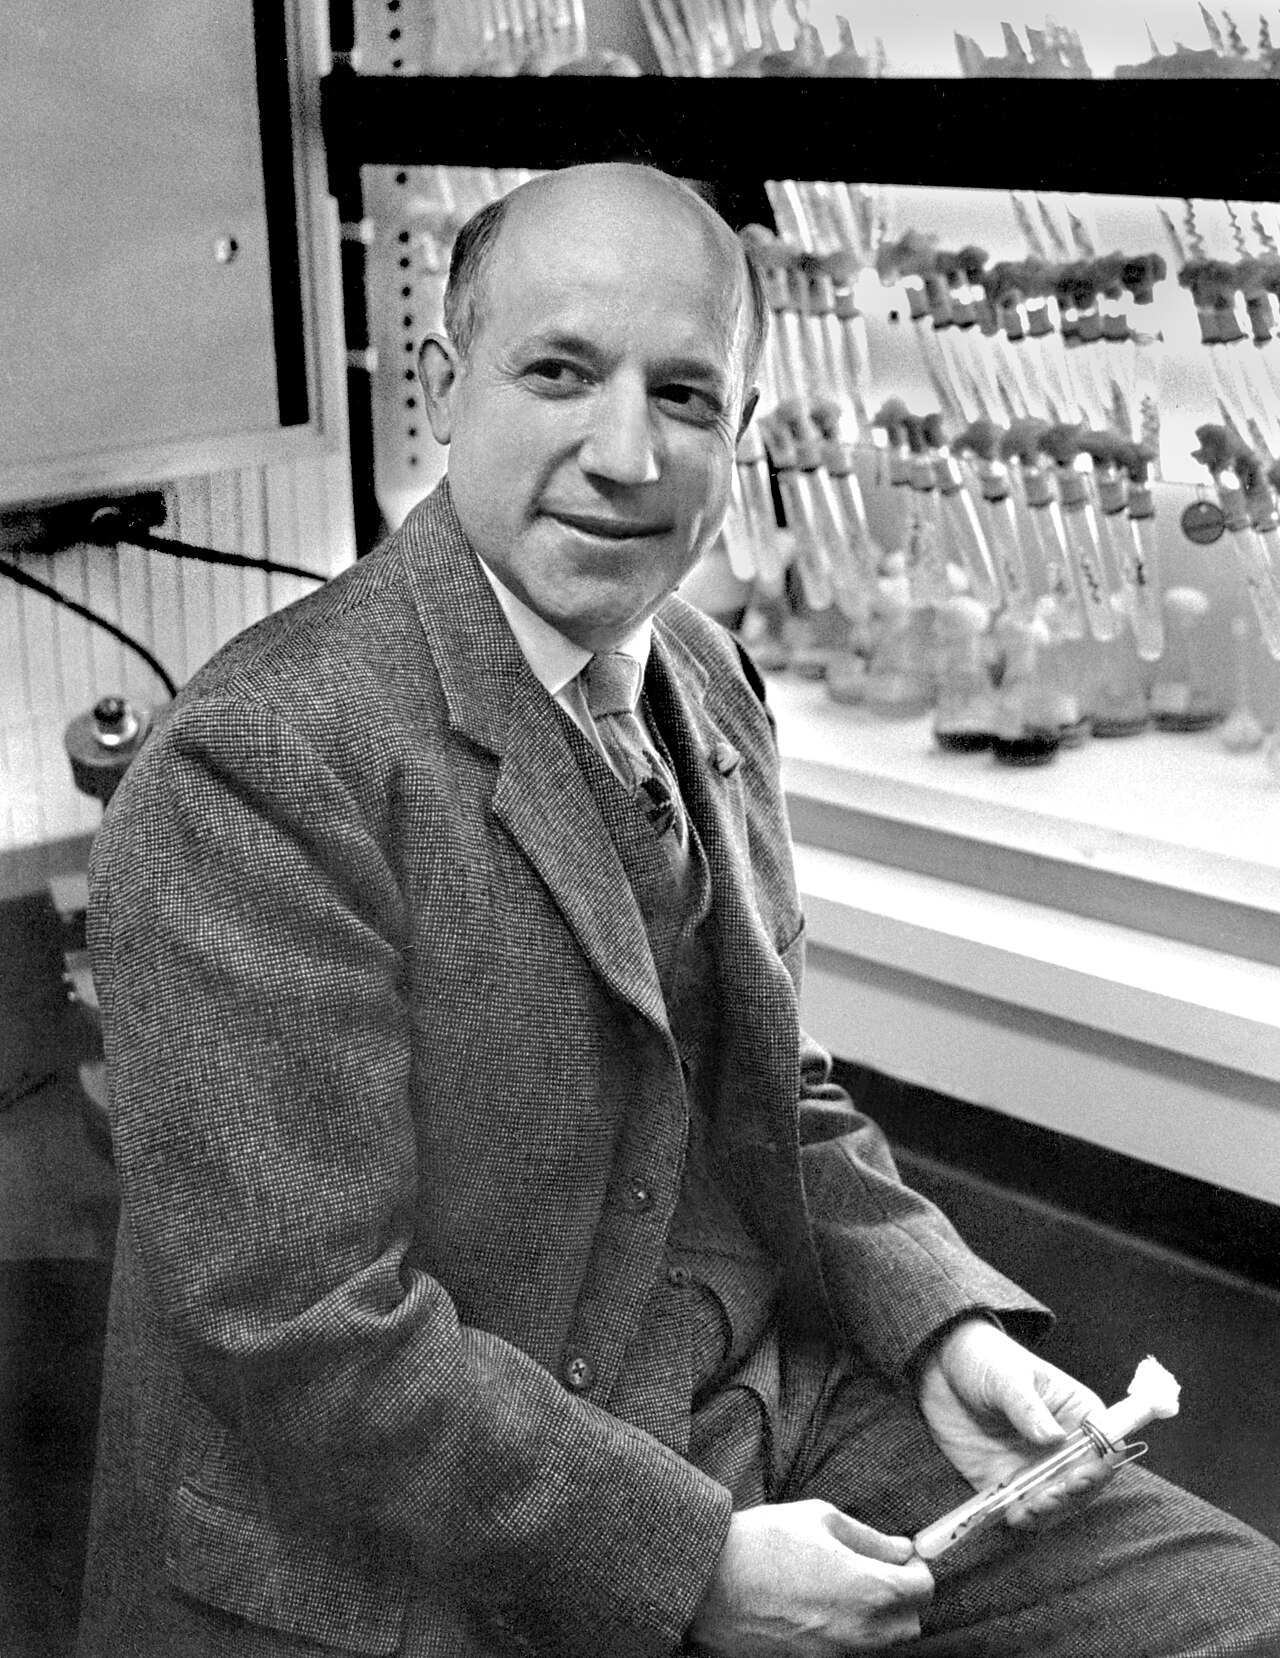
\includegraphics[width=0.26\linewidth]{images/book3/calvin.jpg}

{\small ملفن كالفن (1911--1997)، الذي تتبع مع بنسون مسار الكربون من
$\mathrm{CO_2}$ إلى السكر بكربون مشع واستشراب ورقي. الصورة: Lawrence
Berkeley Laboratory، ملك عام.}
\end{omfigure}

\begin{omfigure}
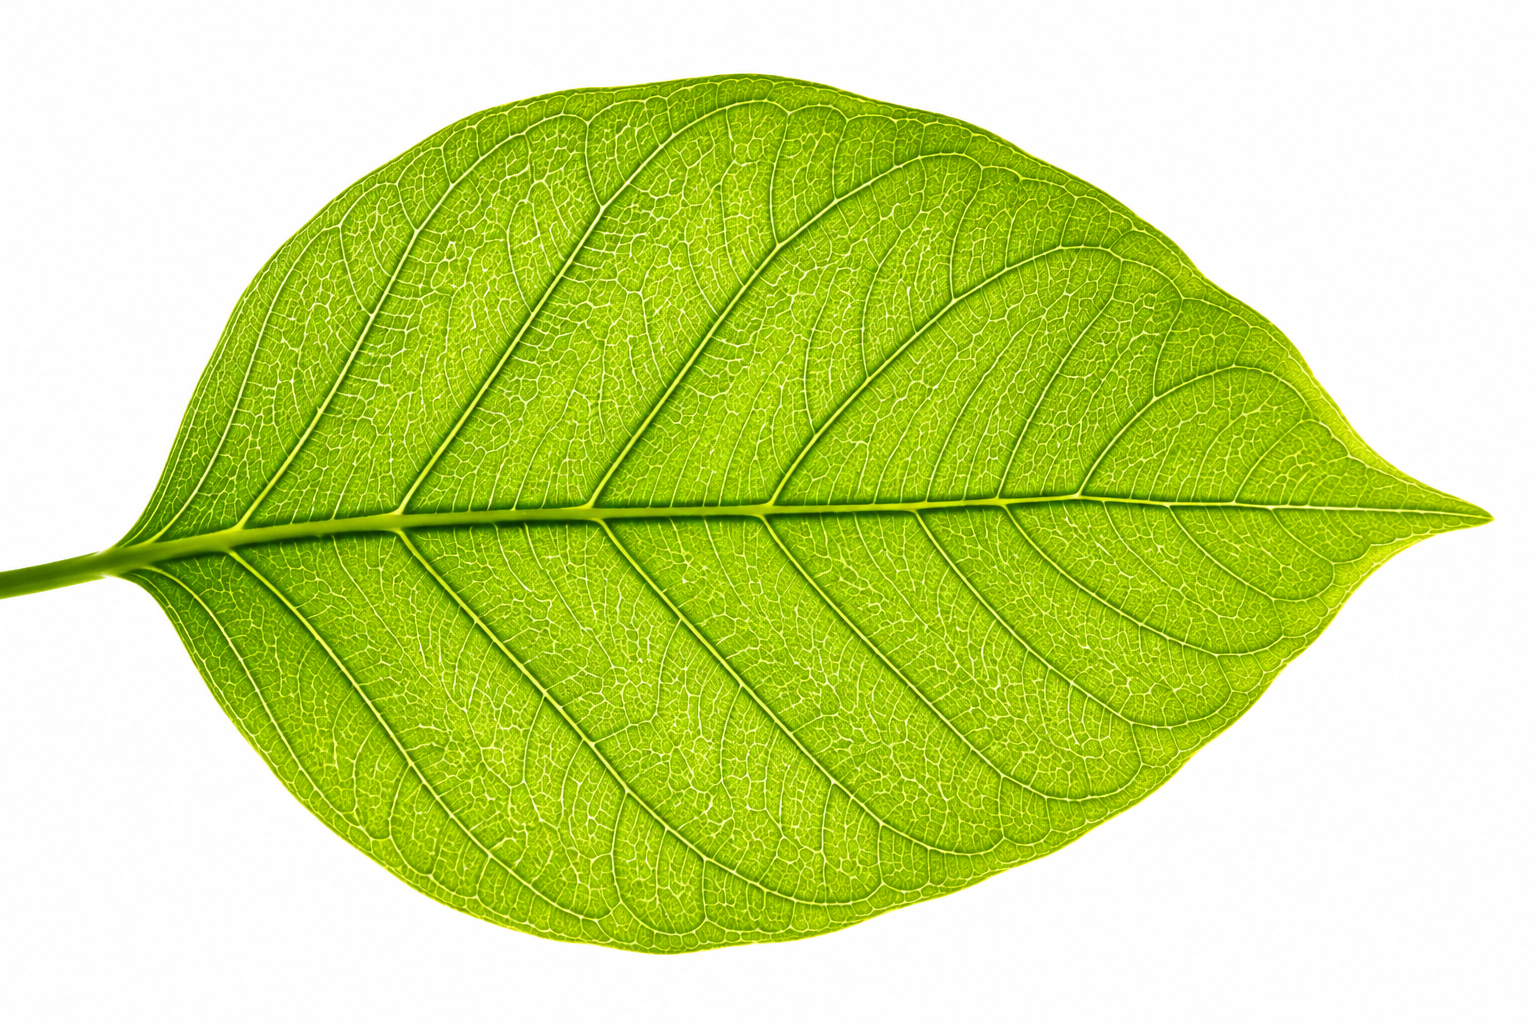
\includegraphics[width=0.6\linewidth]{images/book3/ai/b3-14-leaf-backlit.png}

{\small \omterm{def:b1:flowering-plant-organization:organs}{ورقة} أمام الشمس: الضوء الذي تمتصه يقود، في كل \omterm{def:b1:photosynthesis:chloroplast}{بلاستيدة خضراء}
من خلاياها العمادية، شطر الماء وتثبيت ثاني أكسيد الكربون الذي دخل
عبر ثغورها.}
\end{omfigure}

\begin{method}[موازنة ميزانية تركيب ضوئي]\label{met:b1:photosynthesis:budget}
\begin{enumerate}
  \item عُدّ الكربونات: فكل $\mathrm{CO_2}$ مثبَّت يعطي كربونًا واحدًا
        من الناتج؛ والغلوكوز الواحد يحتاج إلى ست دورات \omterm{def:b1:photosynthesis:fixation}{لروبيسكو}.
  \item عُدّ الحوامل: فكل دورة تكلف 3 \omterm{def:b1:water-small-molecules:atp}{ATP} و2 NADPH (أي 9 و6 لكل
        G3P)؛ والغلوكوز الواحد يكلف 18 \omterm{def:b1:water-small-molecules:atp}{ATP} و12 NADPH.
  \item عُدّ الفوتونات: فالجريان الخطي يعطي 2 NADPH ونحو 3 \omterm{def:b1:water-small-molecules:atp}{ATP} لكل
        $\mathrm{O_2}$، مقابل 8 فوتونات (4 لكل \omterm{def:b1:photosynthesis:zscheme}{نظام ضوئي})؛ و12 NADPH
        تحتاج إلى 6 $\mathrm{O_2}$ و48 فوتونًا؛ \omterm{def:b1:water-small-molecules:atp}{وATP} الزائد يأتي من
        الجريان الحلقي (ببضعة فوتونات أخرى). أي نحو 8 فوتونات لكل
        $\mathrm{CO_2}$: وهو المتطلب الكمي.
  \item عُدّ الطاقة: فمول من فوتونات \qty{680}{nm} هو \qty{176}{kJ}؛
        و48 فوتونًا هي \qty{8450}{kJ} مقابل \qty{2870}{kJ} مخزونة في
        الغلوكوز: أي \qty{34}{\%} على أحسن تقدير، قبل أي فقد بالانعكاس
        والتنفس والجزء غير الممتص من الطيف.
\end{enumerate}
\end{method}

\section{التنفس الضوئي ونباتات C4 وCAM}

\begin{proposition}[عيب روبيسكو]\label{prop:b1:photosynthesis:photorespiration}
\index{التنفس الضوئي}
يقبل \omterm{def:b1:photosynthesis:fixation}{روبيسكو} أيضًا $\mathrm{O_2}$ مكان $\mathrm{CO_2}$: فأكسجة RuBP
تعطي 3-PGA واحدًا وفوسفوغليكولات ثنائي الكربون، وعلى \omterm{def:b1:cell-unit-of-life:cell}{الخلية} أن
تنقذه بطريق مكلف عبر ثلاث \omterm{def:b1:cell-unit-of-life:prokeuk}{عضيات} يطلق $\mathrm{CO_2}$ ويستهلك \omterm{def:b1:water-small-molecules:atp}{ATP} ---
وهو \emph{\omterm{prop:b1:photosynthesis:photorespiration}{التنفس الضوئي}}. \omterm{def:b1:enzymes:enzyme}{والإنزيم} يميز تمييزًا رديئًا (نحو
\qty{80}{} إلى 1 لصالح $\mathrm{CO_2}$ عند تركيزين متساويين)، وفي
الهواء يفوق $\mathrm{O_2}$ غاز $\mathrm{CO_2}$ وفرةً بخمسمئة مرة؛
وعند \qty{25}{\celsius} يضيع ربع عمليات \omterm{def:b1:photosynthesis:fixation}{التثبيت}، وأكثر في الطقس الحار
الجاف حين تنغلق الثغور ويهبط $\mathrm{CO_2}$ داخل \omterm{def:b1:flowering-plant-organization:organs}{الورقة}. \omterm{def:b1:photosynthesis:fixation}{وروبيسكو}،
وقد نشأ حين لم يكن في الهواء أكسجين، بطيء أيضًا (ثلاث دورات في
الثانية) ويُعوَّض بالوفرة: فهو أوفر \omterm{def:b1:proteins:peptide}{بروتين} على الأرض، ونصف \omterm{def:b1:proteins:peptide}{البروتين}
الذواب في \omterm{def:b1:flowering-plant-organization:organs}{ورقة}.
\end{proposition}

\begin{definition}[نباتات C4 وCAM]\label{def:b1:photosynthesis:c4cam}
\index{نبات C4}\index{نبات CAM}
\emph{نباتات C4} (الذرة، وقصب السكر، والذرة الرفيعة، وكثير من
النجيليات المدارية) تسد التسرب بتركيز $\mathrm{CO_2}$: ففي \omterm{def:b1:cell-unit-of-life:cell}{خلايا}
\omterm{def:b1:body-plans-tissues:tissue}{النسيج} الوسطي يثبّت \omterm{def:b1:enzymes:enzyme}{إنزيم} لا ألفة له مع $\mathrm{O_2}$ (كربوكسيلاز
PEP) البيكربونات في \omterm{def:b1:water-small-molecules:ph}{حمض} رباعي الكربون، يُنقل إلى \omterm{def:b1:cell-unit-of-life:cell}{خلايا} \emph{غمد
الحزمة} حول العروق ويُنزع كربوكسيله هناك، فيرتفع $\mathrm{CO_2}$
حول \omterm{def:b1:photosynthesis:fixation}{روبيسكو} عشرة أضعاف وتُقمع الأكسجة --- بكلفة \omterm{def:b1:water-small-molecules:atp}{ATP} زائدين لكل
$\mathrm{CO_2}$. ونوعا \omterm{def:b1:cell-unit-of-life:cell}{الخلايا} يكوّنان تشريح \emph{كرانتس}
(«الإكليل»). أما \emph{نباتات CAM} (الصبّار، والأناناس، والأغاف)
فتفصل الخطوتين نفسيهما في الزمن لا في المكان: فتفتح ثغورها ليلًا،
وتخزن $\mathrm{CO_2}$ حمضَ تفاح في \omterm{def:b1:eukaryotic-cell:plantcell}{الفجوة}، وتطلقه إلى \omterm{def:b1:photosynthesis:fixation}{روبيسكو} نهارًا
وثغورها مغلقة، فتفقد عُشر ما يفقده نبات C3 من ماء لكل كربون مثبَّت.
\end{definition}

\begin{omfigure}
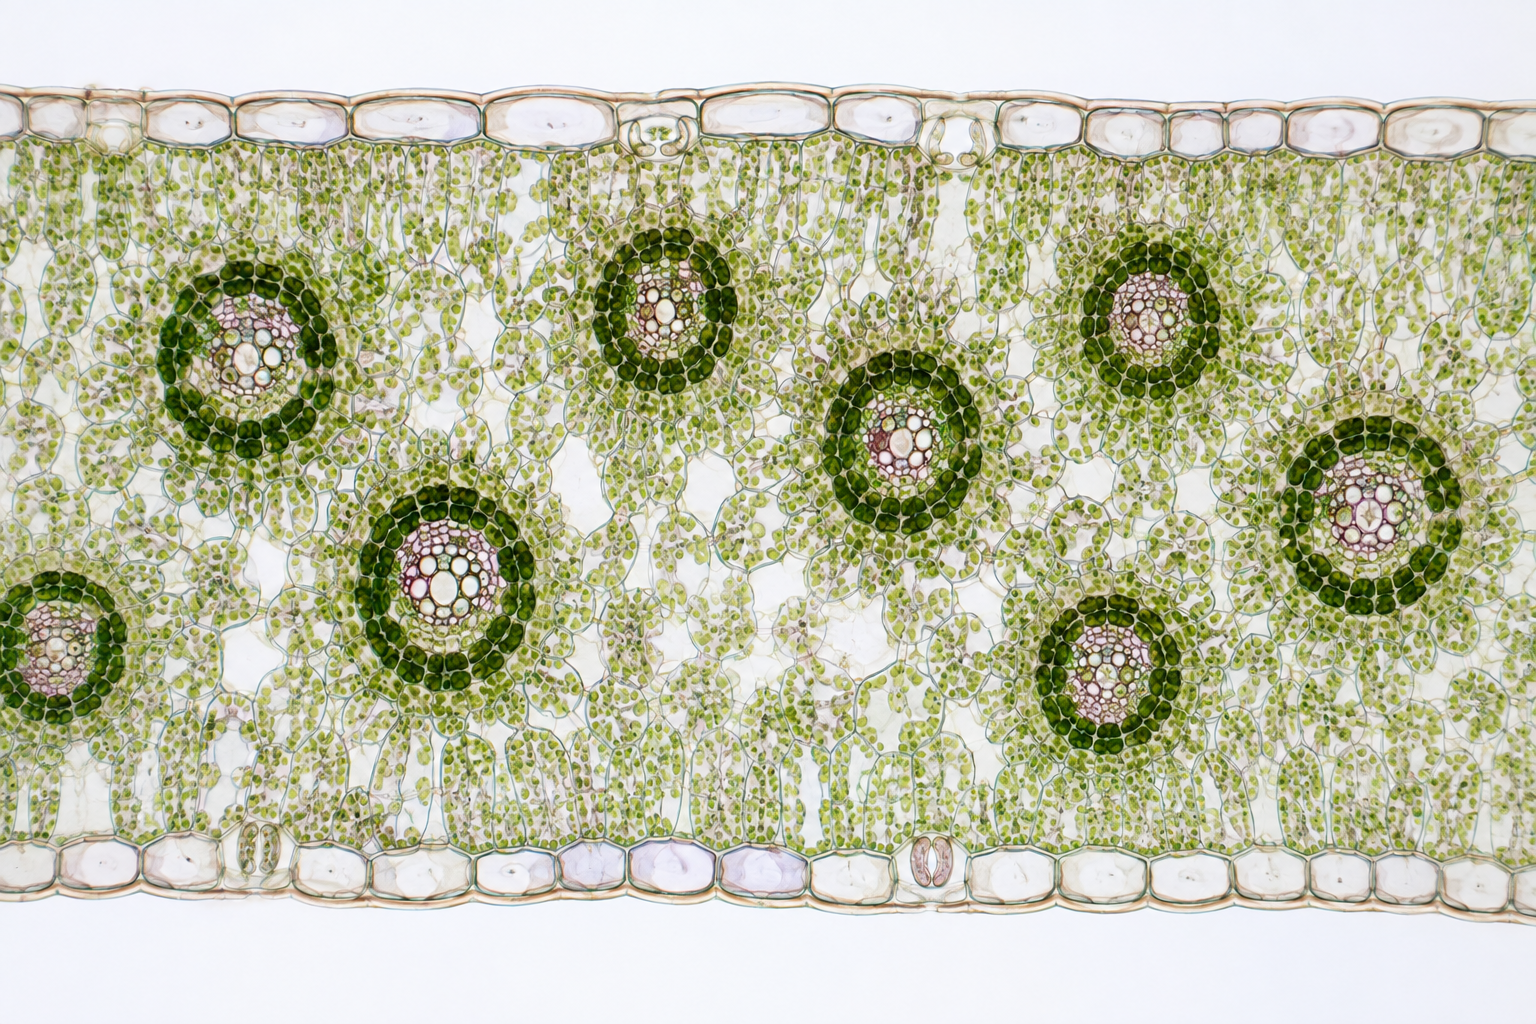
\includegraphics[width=0.6\linewidth]{images/book3/ai/b3-14-maize-kranz.png}

{\small تشريح كرانتس في \omterm{def:b1:flowering-plant-organization:organs}{ورقة} ذرة: كل عرق مكلل \omterm{def:b1:cell-unit-of-life:cell}{بخلايا} غمد حزمة كبيرة
مكتظة \omterm{def:b1:eukaryotic-cell:plastid}{بالبلاستيدات الخضراء}، تحيط بها بدورها \omterm{def:b1:cell-unit-of-life:cell}{خلايا} \omterm{def:b1:body-plans-tissues:tissue}{النسيج} الوسطي.
ويُلتقط $\mathrm{CO_2}$ في الحلقة الخارجية ويُسلَّم، مركَّزًا، إلى
\omterm{def:b1:photosynthesis:fixation}{روبيسكو} في الداخلية.}
\end{omfigure}

\begin{example}[أي نبات أين]\label{ex:b1:photosynthesis:where}
عند \qty{20}{\celsius} في هواء رطب تثبّت \omterm{def:b1:flowering-plant-organization:organs}{ورقة} قمح C3 \omterm{def:b1:flowering-plant-organization:organs}{وورقة} ذرة C4
الكربون بمعدلين متقاربين، وتدفع الذرة \omterm{def:b1:water-small-molecules:atp}{ATP} زائدين لكل كربون. وعند
\qty{35}{\celsius} في هواء جاف يفقد القمح ثلث تثبيته للتنفس الضوئي
بينما لا تفقد الذرة شيئًا: فنجيليات C4 تسيطر على البلاد الحارة
المكشوفة، ونباتات C3 على الباردة والمظللة. أما الصبّار فيثبّت ببطء
بالمعيارين كليهما لكنه ينجو حيث تموت الأخرى عطشًا.
\end{example}

\section{التغذي الذاتي}

\begin{definition}[التغذي الذاتي]\label{def:b1:photosynthesis:autotrophy}
يكون الكائن \emph{ذاتي التغذي}\index{التغذي الذاتي} حين يبني مادته
العضوية من $\mathrm{CO_2}$ (\cref{ch:b1:organism-environment}). وهو
يحتاج إلى منبع طاقة ومنبع إلكترونات. \emph{\omterm{def:b1:organism-environment:trophy}{فذاتيات التغذي الضوئية}}
تأخذ الطاقة من الضوء: فالنباتات والطحالب والبكتيريا الزرقاء تأخذ
إلكتروناتها من الماء وتطلق الأكسجين (\emph{مطلقة للأكسجين})؛
والبكتيريا الأرجوانية والخضراء تأخذها من كبريتيد الهيدروجين أو من
حموض عضوية ولا تطلق شيئًا. و\emph{\omterm{def:b1:organism-environment:trophy}{ذاتيات التغذي الكيميائية}} تأخذ
الطاقة والإلكترونات معًا من أكسدة مركبات معدنية --- النشادر،
والنتريت، والكبريتيد، والهيدروجين، والحديد الثنائي --- بلا ضوء
البتة: كبكتيريا الأزوتة في التربة، والبكتيريا التي تغذي أنظمة فوهات
الأعماق. وكلها تستعمل \omterm{def:b1:photosynthesis:fixation}{دورة كالفن}، أو دورة قريبة منها، لتثبيت
الكربون؛ وكلها ترجعه بجزيء NADPH وتدفع بجزيء \omterm{def:b1:water-small-molecules:atp}{ATP}؛ ولا تختلف إلا في مصدر \omterm{def:b1:water-small-molecules:atp}{ATP}
والإلكترونات.
\end{definition}

\begin{example}[الميزانية العالمية]\label{ex:b1:photosynthesis:global}
يثبّت التركيب الضوئي نحو \qty{120}{Gt} من الكربون في السنة على
اليابسة و\qty{50}{Gt} في المحيطات، نصفها بطحالب وحيدة \omterm{def:b1:cell-unit-of-life:cell}{الخلية}
وبكتيريا زرقاء لا تراها العين؛ وهو يقلّب ثاني أكسيد كربون الجو كل
سبع سنين وأكسجينه كل ألفي سنة. والأكسجين جاء بالطريق نفسه: فمليارَي
سنة أطلقته البكتيريا الزرقاء في جو لم يكن فيه شيء منه، وكل كائن
هوائي، من \omterm{def:b1:eukaryotic-cell:mitochondrion}{المتقدرة} صعودًا، مبني على تسرب جملة إنزيمية واحدة تشطر
الماء.
\end{example}

\section{تمارين}

\begin{exercise}[$\star$]\label{exo:b1:photosynthesis:1}
سمِّ جمل \omterm{def:b1:membranes-transport:membrane}{الأغشية} الثلاث في \omterm{def:b1:photosynthesis:chloroplast}{البلاستيدة الخضراء} وقل أين تجري \omterm{prop:b1:photosynthesis:lightreactions}{التفاعلات
الضوئية} وأين تجري \omterm{def:b1:photosynthesis:fixation}{دورة كالفن}.
\end{exercise}

\begin{exercise}[$\star$]\label{exo:b1:photosynthesis:2}
اكتب معادلة \omterm{prop:b1:photosynthesis:lightreactions}{التفاعلات الضوئية} وقل من أين يأتي الأكسجين المطلق، مع
الشاهد.
\end{exercise}

\begin{exercise}[$\star$]\label{exo:b1:photosynthesis:3}
سمِّ مراحل \omterm{def:b1:photosynthesis:fixation}{دورة كالفن} الثلاث وعدد \omterm{def:b1:water-small-molecules:atp}{ATP} وNADPH المستهلكين لكل
$\mathrm{CO_2}$ مثبَّت.
\end{exercise}

\begin{exercise}[$\star$]\label{exo:b1:photosynthesis:4}
من شكل الأطياف، عند أي أطوال موجة يمتص \omterm{def:b1:photosynthesis:pigments}{اليخضور} $a$ أكثر ما يمتص،
ولماذا كان طيف الفعل أعلى من امتصاص \omterm{def:b1:photosynthesis:pigments}{اليخضور} حول \qty{500}{nm}؟
\end{exercise}

\begin{exercise}[$\star\star$]\label{exo:b1:photosynthesis:5}
فسّر أثر إمرسون في التعزيز وما الذي كشفه عن تنظيم \omterm{prop:b1:photosynthesis:lightreactions}{التفاعلات الضوئية}.
\end{exercise}

\begin{exercise}[$\star\star$]\label{exo:b1:photosynthesis:6}
قوة محركة للبروتون قدرها \qty{0.18}{V} تقابل كم طاقة حرة لكل مول
بروتون ($F = \qty{96500}{C/mol}$)؟ وكم بروتونًا يجب أن يجري لصنع
\omterm{def:b1:water-small-molecules:atp}{ATP} واحد عند \qty{50}{kJ/mol}؟ قارن مع الأربعة التي يستعملها
السنتاز.
\end{exercise}

\begin{exercise}[$\star\star$]\label{exo:b1:photosynthesis:7}
صنعت ثايلاكويدات ياغندورف \omterm{def:b1:water-small-molecules:atp}{ATP} في الظلام بعد حمام حمضي. فسّر ما الذي
يثبته هذا وما الذي لا يثبته، وتنبأ بالنتيجة لو أُضيف فاصل اقتران قبل
النقل.
\end{exercise}

\begin{exercise}[$\star\star$]\label{exo:b1:photosynthesis:8}
تتبع الكربون: انطلاقًا من 3 RuBP (15 كربونًا) و3 $\mathrm{CO_2}$،
عُدّ الكربونات عبر 3-PGA وG3P وG3P المصدَّر وRuBP المجدد، وتحقق من
الميزان.
\end{exercise}

\begin{exercise}[$\star\star$]\label{exo:b1:photosynthesis:9}
في تجربة كالفن يرتفع RuBP ويهبط 3-PGA حين يُزال $\mathrm{CO_2}$؛
ويرتفع 3-PGA ويهبط RuBP حين يُطفأ الضوء. فسّر الأمرين من الدورة.
\end{exercise}

\begin{exercise}[$\star\star\star$]\label{exo:b1:photosynthesis:10}
احسب طاقة مول من فوتونات \qty{680}{nm} ($h =
\qty{6.63e-34}{J.s}$،
و$c = \qty{3.0e8}{m/s}$، و$N_A = \num{6.02e23}$)، وطاقة الفوتونات
الثمانية والأربعين اللازمة لكل غلوكوز، ومردود خزن \qty{2870}{kJ/mol}.
ولماذا كان مردود محصول كامل، وهو نحو \qty{1}{\%} من ضوء الشمس، أدنى
بكثير؟
\end{exercise}

\begin{exercise}[$\star\star\star$]\label{exo:b1:photosynthesis:11}
عند \qty{25}{\celsius} في الهواء يؤكسج \omterm{def:b1:photosynthesis:fixation}{روبيسكو} مرة واحدة مقابل كل
ثلاث كربكسات؛ وكل أكسجة تطلق نصف $\mathrm{CO_2}$ في الإنقاذ وتكلف
\omterm{def:b1:water-small-molecules:atp}{ATP}. احسب الكربون الصافي المثبَّت لكل 100 كربكسة والكسر الضائع.
\omterm{def:b1:photosynthesis:c4cam}{ونبات C4} يتجنب الفقد لكنه ينفق 2 \omterm{def:b1:water-small-molecules:atp}{ATP} زائدين لكل $\mathrm{CO_2}$:
فعند أي كسر من الفقد يسدد تصميم C4، إذا كان \omterm{def:b1:water-small-molecules:atp}{ATP} الواحد يساوي نحو
عُشر $\mathrm{CO_2}$ مثبَّت؟
\end{exercise}

\begin{exercise}[$\star\star\star$]\label{exo:b1:photosynthesis:12}
«التركيب الضوئي تنفس يجري بالمقلوب.» ناقش في فقرة، مقارنًا الآلية
التناضحية الكيميائية، واتجاه جريان الإلكترونات، والحوامل، والدورات،
وقل أين تصدق المشابهة وأين تفشل.
\end{exercise}

\section{مسألة: ثمن جزيء غلوكوز}

\begin{problem}[{مسألة نهاية الأسبوع --- فوتونات معدودة، وإلكترونات
وبروتونات متتبَّعة عبر الثايلاكويد، وATP وNADPH محسوبان ومنفقان،
وحصاد ورقة يومي موزون، وصولًا إلى المردود الطاقي للتركيب الضوئي}]
\label{pb:b1:photosynthesis:1}
الثوابت: $h = \qty{6.63e-34}{J.s}$، و$c = \qty{3.00e8}{m/s}$،
و$N_A = \num{6.02e23}$، و$F = \qty{96500}{C/mol}$، و$R = \qty{8.314}{J.mol^{-1}.K^{-1}}$،
و$T = \qty{298}{K}$. \omterm{prop:b1:water-small-molecules:gibbs}{والطاقة الحرة} لاحتراق الغلوكوز
\qty{2870}{kJ/mol}؛ وتركيب \omterm{def:b1:water-small-molecules:atp}{ATP} في \omterm{def:b1:eukaryotic-cell:plastid}{البلاستيدة} يكلف
\qty{50}{kJ/mol}؛ وNADPH يحمل \qty{220}{kJ/mol} من القدرة المرجعة.

\medskip
\noindent\textbf{الجزء الأول --- الفوتونات والإلكترونات.}
\begin{enumerate}
  \item احسب طاقة فوتون واحد عند \qty{680}{nm} وطاقة مول منها.
  \item احسب طاقة مول من فوتونات \qty{700}{nm} ومن فوتونات
        \qty{450}{nm}. ولماذا لا يعطي الضوء الأزرق تركيبًا ضوئيًا
        أكثر لكل فوتون من الأحمر؟
  \item كم فوتونًا من \qty{680}{nm} يحمل جولًا واحدًا؟
  \item نقل إلكترون واحد من الماء ($E'_0 = \qty{+0.82}{V}$) إلى
        $\mathrm{NADP^+}$ ($E'_0 = \qty{-0.32}{V}$) يقتضي كم طاقة حرة
        لكل مول إلكترونات ($\Delta G = -nF\Delta E$)؟
  \item يُستعمل فوتونان لكل إلكترون (واحد في كل \omterm{def:b1:photosynthesis:zscheme}{نظام ضوئي}). احسب
        الطاقة المزوَّدة لكل مول إلكترونات والكسر المخزون منها في تغير
        الأكسدة والإرجاع.
  \item كم إلكترونًا، ومن ثم كم فوتونًا، يلزم لصنع $\mathrm{O_2}$
        واحد وجزيئي NADPH؟
  \item وكم فوتونًا لكل غلوكوز، إذا لزم 12 NADPH؟
\end{enumerate}

\medskip
\noindent\textbf{الجزء الثاني --- البروتونات \omterm{def:b1:water-small-molecules:atp}{وATP}.}
لكل $\mathrm{O_2}$ مطلق، تتحرر أربعة بروتونات في اللمعة بشطر الماء
وتُضخ ثمانية بمعقد السيتوكروم $b_6f$؛ \omterm{thm:b1:photosynthesis:chemiosmosis}{وسنتاز ATP} يستعمل
\qty{4}{H^+} لكل \omterm{def:b1:water-small-molecules:atp}{ATP}. واللمعة عند pH 5 \omterm{def:b1:photosynthesis:chloroplast}{والسدى} عند pH 8؛ \omterm{def:b1:membranes-transport:potential}{وكمون الغشاء}
عبر \omterm{def:b1:photosynthesis:chloroplast}{الثايلاكويد} مهمل.
\begin{enumerate}[resume]
  \item احسب القوة المحركة للبروتون من فرق pH، بالفولط
        ($\Delta\mu = 2.303\,RT\,\Delta\mathrm{pH}/F$)، \omterm{prop:b1:water-small-molecules:gibbs}{والطاقة الحرة}
        لكل مول بروتون.
  \item احسب البروتونات المسلَّمة إلى اللمعة لكل $\mathrm{O_2}$ \omterm{def:b1:water-small-molecules:atp}{وATP}
        الذي تستطيع صنعه.
  \item احسب \omterm{def:b1:water-small-molecules:atp}{ATP} المصنوع لكل غلوكوز بالجريان الخطي (6
        $\mathrm{O_2}$)، وقارنه بالثمانية عشر التي تحتاجها \omterm{def:b1:photosynthesis:fixation}{دورة
        كالفن}. وكيف يُسدّ النقص؟
  \item احسب \omterm{prop:b1:water-small-molecules:gibbs}{الطاقة الحرة} المتاحة من البروتونات لكل \omterm{def:b1:water-small-molecules:atp}{ATP}
        (\qty{4}{H^+}) ومردود السنتاز.
  \item حجم لمعة \omterm{def:b1:photosynthesis:chloroplast}{بلاستيدة خضراء} نحو \qty{1}{\micro m^3}. فكم بروتونًا
        حرًا تحمل عند pH 5؟ قارن مع نحو $10^5$ بروتون تعبر السنتازات
        كل ثانية، واستنتج ما الذي يهدّئ اللمعة.
\end{enumerate}

\medskip
\noindent\textbf{الجزء الثالث --- السكر.}
\begin{enumerate}[resume]
  \item اكتب الطاقة المخزونة لكل غلوكوز بوصفها 18 \omterm{def:b1:water-small-molecules:atp}{ATP} $\times$
        \qty{50}{kJ} زائد 12 NADPH $\times$ \qty{220}{kJ}، وقارنها
        بمقدار \qty{2870}{kJ} في الغلوكوز. فأين يذهب الفرق؟
  \item احسب طاقة الفوتونات الثمانية والأربعين في السؤال 6 ومردود
        التركيب الضوئي من الفوتون إلى الغلوكوز.
  \item \qty{45}{\%} فقط من ضوء الشمس في أطوال الموجة التي تمتصها
        الأصبغة، وعُشر ذلك ينعكس أو ينفذ. احسب المردود من ضوء الشمس
        الساقط إلى الغلوكوز، قبل التنفس.
  \item \omterm{def:b1:flowering-plant-organization:organs}{ورقة} مساحتها \qty{50}{cm^2} تتلقى \qty{400}{W/m^2} من ضوء
        الشمس \qty{10}{h}. احسب الطاقة المتلقاة، ثم الغلوكوز المصنوع
        بالغرام عند مردود السؤال 14 (\qty{180}{g/mol}).
  \item تتنفس \omterm{def:b1:flowering-plant-organization:organs}{الورقة} \qty{40}{\%} من ذلك الغلوكوز لتبقى حية. فما
        كسبها الصافي، بغرامات الغلوكوز وبغرامات الكربون؟
  \item يبلغ محصول \qty{1}{\%} مردودًا إجماليًا في موسم. اذكر ثلاثة
        فواقد، غير ما حُسب، تفصل رقم \omterm{def:b1:flowering-plant-organization:organs}{الورقة} عن رقم المحصول.
\end{enumerate}

\medskip
\noindent\textbf{الجزء الرابع --- التسرب.}
\omterm{def:b1:photosynthesis:fixation}{روبيسكو} في الهواء عند \qty{25}{\celsius} يجري أكسجة واحدة لكل ثلاث
كربكسات؛ وكل أكسجة تكلف ما يعادل نصف $\mathrm{CO_2}$ مثبَّت
و3.5 \omterm{def:b1:water-small-molecules:atp}{ATP}.
\begin{enumerate}[resume]
  \item لكل 100 كربكسة، احسب الأكسجات، والكربون الضائع، والكربون
        الصافي المكتسب.
  \item احسب \omterm{def:b1:water-small-molecules:atp}{ATP} المنفق على الإنقاذ لكل 100 كربكسة ومجموع \omterm{def:b1:water-small-molecules:atp}{ATP} لكل
        كربون صافٍ مكتسب (3 \omterm{def:b1:water-small-molecules:atp}{ATP} \omterm{def:b1:photosynthesis:fixation}{لدورة كالفن} لكل كربكسة زائد
        الإنقاذ).
  \item \omterm{def:b1:photosynthesis:c4cam}{نبات C4} لا أكسجة له لكنه ينفق 2 \omterm{def:b1:water-small-molecules:atp}{ATP} زائدين لكل
        $\mathrm{CO_2}$ مسلَّم. احسب \omterm{def:b1:water-small-molecules:atp}{ATP} لكل كربون صافٍ عنده وقارن.
  \item عند \qty{35}{\celsius} ترتفع نسبة الأكسجة إلى واحدة لكل
        اثنتين. أعد حساب أرقام C3 وقل أي تصميم يفوز.
  \item فسّر لماذا يرفع رفع $\mathrm{CO_2}$ في دفيئة إلى ثلاثة أمثال
        القيمة الجوية مردودَ محاصيل C3 (الطماطم، والقمح) ولا يكاد يرفع
        مردود محاصيل C4 (الذرة).
  \item \omterm{def:b1:flowering-plant-organization:organs}{ورقة} C3 تفقد نحو 250 جزيء ماء لكل $\mathrm{CO_2}$ مثبَّت،
        \omterm{def:b1:photosynthesis:c4cam}{ونبات CAM} نحو 25. احسب الماء الذي يفقده كل منهما لتثبيت
        \qty{1}{g} من الكربون.
  \item اذكر النتيجة: المتطلب الكمي لكل $\mathrm{CO_2}$، والمردود من
        الفوتون إلى الغلوكوز، والمردود من ضوء الشمس إلى سكر \omterm{def:b1:flowering-plant-organization:organs}{الورقة}
        الصافي.
\end{enumerate}
\end{problem}
